%!TEX root = PMP_ClockPendulumAnalyzer.tex
\section{Projektorganisation}
    Das Projekt besteht aus 2 Entwicklern und einem Auftraggeber der als Ansprechperson gilt. Dadurch wird die Projektorganisation möglichst leicht gehalten. Die Verantwortung wird gleichmässig auf die beiden Entwickler aufgeteilt.
    \begin{figure}[H]
        \centering
        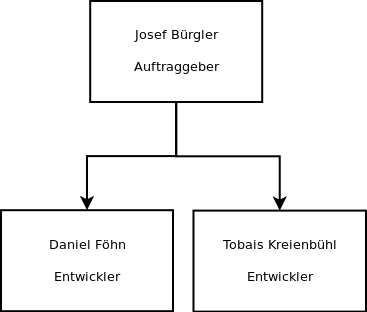
\includegraphics[width=.5\textwidth]{organisation.png}
        \caption{einfache Projektorganisationsstruktur}
    \end{figure}
	\textbf{Entwickler:} Tobias Kreienbühl
    \begin{itemize}
        \item Projektplanung
        \item Entwicklung der Software
        \item Entwicklung der Mechanik
        \item Mathematische Umsetzung
    \end{itemize}
    \vspace{.5cm}
    \textbf{Entwickler:} Daniel Föhn
    \begin{itemize}
        \item Projektplanung
        \item Entwicklung der Software
        \item Entwicklung der Elektronik
        \item Aufbau der Environment
    \end{itemize}
    \vspace{.5cm}
    \textbf{Auftraggeber:} Josef Bürgler
    \begin{itemize}
        \item Anforderungen abnehmen
        \item 
    \end{itemize}